

\newpage
\section{21-03-2019: COLLECTION, LIST E SET}
\begin{center}
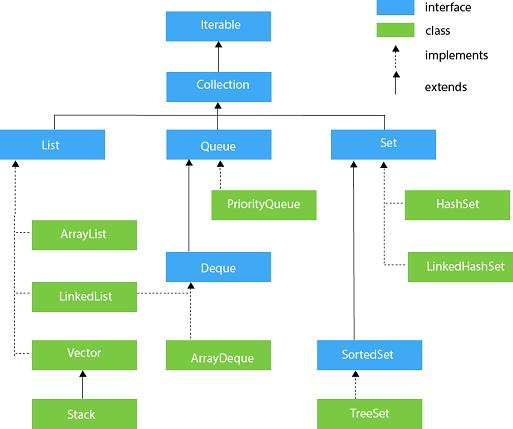
\includegraphics[width=%
0.6\textwidth]{java-collection-hierarchy}
\end{center} 

\begin{center}
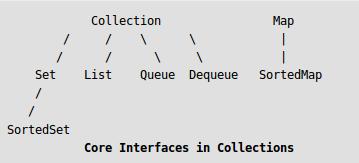
\includegraphics[width=%
0.6\textwidth]{MapInterface}
\end{center} 
\textbullet\ -> ITERABLE:Posso solo scorrere \newline
\textbullet\ ---> COLLECTION: Posso scorrere, aggiungere e togliere \newline
\textbullet\ -----> LIST: Posso scorrere e aggiungere o togliere con un indice \newline
\textbullet\ -------> ARRAYLIST:è sottotipo di list, in quanto implementa list! \newline
\digraph{ao}{rankdir=LR;

   a [label="Iterable" shape = "record"]; 
   b [label="Collection" shape = "record"]; 
   c [label="Set" shape = "record"]; 
   d [label="Hash" shape = "record"]; 
   e [label="List" shape = "record"]; 
   f [label="ArrayList" shape = "record"];    
   b->a; e->b; f->e; d->c; c->b} \newline

\noindent Per evitare di riprodurre codice si usano le classi astratte dalle quali poi si erediterà. 

\noindent Relazione di ordinamento: operatore binario che permette di mappare elementi di due insiemi diversi.

\noindent Una classe con metodi tutti statici non si può costruire. Rappresenta dunque un contenitore di metodi (è un pezzo di libreria).

\noindent \textbf{CARATTERISTICHE DI SET}\newline
\textbullet\ Gli elementi non sono duplicati \newline
\textbullet\ Gli elementi non sono ordinati in base a come sono inseriti \newline	
\textbullet\ Non vengono inseriti metodi nuovi, eredita solo quelli del padre \newline
\textbullet\ I metodi nuovi vengono messi nella classe che implementa l'interfaccia \newline
\textbullet\ Tiene un ordinamento che cerca di massimizzare le operazioni di ricerca ed estrazione \newline

\noindent \textbf{CARATTERISTICHE DI LIST}\newline
\textbullet\ Gli elementi possono essere duplicati \newline
\textbullet\ Gli elementi sono ordinati in base all'ordine di inserimento \newline	
\textbullet\ Rispetto ai metodi del padre ne aggiunge altri che permettono di leggere ed inserire elementi in un determinato indice \newline

\noindent \textbf{CODICE DI ESEMPIO}\newline
Il professore questo giorno ha caricato su github del codice chiamato: TinyJDK. Lo riporto per completezza:
\begin{lstlisting}[basicstyle=\small,]
/* Classe: MyIterable.java */
public interface MyIterable<E> {

    MyIterator<E> iterator();
    int find(E x) throws Exception;

}
\end{lstlisting}

\begin{lstlisting}[basicstyle=\small,]
/* Classe: MyIterator.java */
public interface MyIterator<E> {
    boolean hasNext();
    E next();
}
\end{lstlisting}

\begin{lstlisting}[basicstyle=\small,]
/* Classe: MyCollection.java */
import java.util.Collection;
import java.util.function.Function;

public interface MyCollection<T> extends MyIterable<T> {
    void add(T x);
    void clear();
    void remove(T x);   // da decidere se ci piace o no
    boolean contains(T x);
    boolean contains(Function<T, Boolean> p);
    int size();


}
\end{lstlisting}

\begin{lstlisting}[basicstyle=\small,]
/* Classe: MyList.java */

public interface MyList<T> extends MyCollection<T> {
    void add(int i, T x);
    T get(int i);
    void set(int i, T x);
}
\end{lstlisting}

\begin{lstlisting}[basicstyle=\small,]
/* Classe: MySet.java */
public interface MySet<T> extends MyCollection<T> {
}
\end{lstlisting}

\noindent \textbf{ESEMPIO IMPLEMENTAZIONE LIST}\newline
Vediamo un esempio di implementazione della classe List, collection in cui gli elementi vengono memorizzati in ordine di arrivo.

\begin{lstlisting}[basicstyle=\small,]
/* Classe: MyArrayList.java */
import java.util.Collection;
import java.util.function.Function;

public class MyArrayList<T> implements MyList<T> {

    private Object[] a;
    private int actualSize;

    public static class MyException extends Exception {
        public MyException(String s) {
            super(s);
        }
    }

/*    T[] toArray() {
        return (T[]) a;
    }*/

/*    public static Exception returnNow() {
        return new Exception("msg");
    }

    public static void throwNow() throws Exception {
        throw new Exception("msg");
    }

    public static void caller() throws Exception {
        Exception e = returnNow();
        throwNow();
    }

    public static void caller2() {
        try {
            caller();
        }
        catch (Exception e2) {
            // fai qualcosa con e2
        }

    }

    public void m(int x) throws Exception {
        MyException e = new MyException("error messagge");
        if (x < 0) throw e;
    }
  */

    public MyArrayList() {
        clear();
    }

    public static class NotFoundException extends Exception {
    }

	/* ritorna l'indice in cui è memorizzato un oggetto
	 * equivalente a quello passato come parametro di 
	 * ingresso */
    @Override
    public int find(T x) throws NotFoundException {
        int cnt = 0;
        MyIterator<T> it = iterator();
        while (it.hasNext())
        {
            T y = it.next();
            if (x.equals(y)) return cnt;
            ++cnt;
        }
        throw new NotFoundException();
    }




    public static void main3() {
        MyArrayList<Integer> c = new MyArrayList<>();
        try {
            int index = c.find(6);
            System.out.println("found at index = " + index);
        } catch (NotFoundException e) {
            try {
                int index = c.find(7);
            } catch (NotFoundException e1) {

            }

        }
    }

    @Override
    public boolean contains(T x) {
        for (int i = 0; i < actualSize; ++i) {
            Object o = a[i];
            if (o.equals(x)) return true;
        }
        return false;
    }


    @Override
    public boolean contains(Function<T, Boolean> p) {
        return false;
    }

    @Override
    public int size() {
        return actualSize;
    }


    @Override
    public void clear() {
        a = new Object[100];
        actualSize = 0;
    }

    @Override
    public void add(T o) {
        a[actualSize++] = o;
        if (actualSize >= a.length) {
            Object[] u = new Object[a.length * 2];
            for (int j = 0; j < a.length; ++j)
                u[j] = a[j];
            a = u;
        }
    }

    @Override
    public MyIterator<T> iterator() {
        return new MyIterator<T>() {
            private int pos = 0;

            @Override
            public boolean hasNext() {
                return pos <= actualSize;
            }

            @Override
            public T next() {
                return (T) MyArrayList.this.a[pos++];
            }
        };
    }

    @Override
    public void add(int i, T x) {

    }

    @Override
    public T get(int i) {
        return (T) a[i];
    }

    @Override
    public void set(int i, T x) {
        a[i] = x;
    }

    @Override
    public void remove(T x) {

    }

}
\end{lstlisting}

\noindent \textbf{ESEMPIO IMPLEMENTAZIONE SET}\newline
Vediamo un esempio di implementazione della classe Set, collection in cui gli elementi vengono inseriti secondo una certa logica interna. In questo caso gli elementi verranno tenuti secondo l'ordine imposto o da comparator o da comparable.

\begin{lstlisting}[basicstyle=\small,]
/* Classe: MyArrayListSet.java */
import java.util.ArrayList;
import java.util.Arrays;
import java.util.Collections;
import java.util.Comparator;
import java.util.function.Function;

public class MyArrayListSet<T extends Comparable<T>> implements MySet<T> {
    private final Comparator<T> p;
    private final ArrayList<T> a;

    public MyArrayListSet(Comparator<T> p) {
        this.a = new ArrayList<T>();
        this.p = p;
    }

    @Override
    public void add(T x) {
        if (!contains(x)) {
            a.add(x);
            sort();
        }
    }

    private void sort() {
        Collections.sort(a, p);
    }

    @Override
    public void clear() {
        a.clear();
    }

    @Override
    public void remove(T x) {
        a.remove(x);
    }

    @Override
    public boolean contains(T x) {
        return a.contains(x);
    }

    @Override
    public boolean contains(Function<T, Boolean> p) {
        return a.contains(p);
    }

    @Override
    public int size() {
        return a.size();
    }

    @Override
    public MyIterator<T> iterator() {
        return a.iterator();
    }

    @Override
    public int find(T x) throws Exception {
        return a.find(x);
    }
}
\end{lstlisting}





